\documentclass[12pt]{article}
\usepackage{hyperref}
\usepackage{graphicx}
\usepackage{mathtools}
\usepackage[margin=1in, paperwidth=8.5in, paperheight=11in]{geometry}
\begin{document}
\title{Istanbul Technical University- Spring 2017 \\ BLG527E Machine Learning \\ Homework 3}
\author{Omid Abdollahi Aghdam \\
student number: 504151520\\
\href{mailto:abdollahi15@itu.edu.tr}{abdollahi15@itu.edu.tr}\\
\href{mailto:abdollahi.omid@gmail.com}{abdollahi.omid@gmail.com}
}
\date{\today}
\maketitle
\newpage
\textbf{Note:} Running hw3.py file will output the result on terminal (linux, MacOsx) or command prompt (Windows). Source codes lines are referenced in report. In addition to hw3.py, hw3.ipynb is also provided.\\

\textbf{Q1)}  
\textbf{Spliting optdigits.tra:} Training set (optdigits.tra) is randomly divided into 90\% train and 10\% validation sets (line 34).\\*

\textbf{knn hyper-parameters tuning:} Best k is selected based on validation accuracy, and corresponding metric will be printed on terminal (lines 94-121).\\*

\textbf{Training with best k on the whole training set:} We train on whole data and report confusion matrix of train set (lines 125-134). It is shown in Figure \ref{fig:knntrain}. This part of source code will output train time and confusion matrix on terminal.
\begin{figure}[h] 
	\begin{center}
		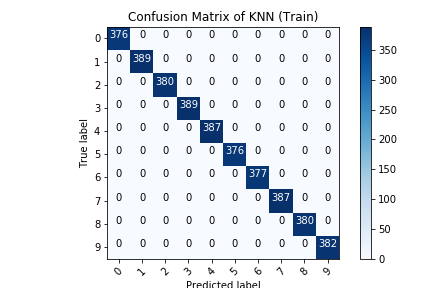
\includegraphics[width=3in]{knntrain.png}
		\caption{Confusion Matrix of Train set (knn).}
		\label{fig:knntrain}
	\end{center}
\end{figure} 

\textbf{Evaluating knn model on test set:} In lines 138-147, we predict test labels and report the metrics. Test set confusion matrix is shown in Figure \ref{fig:knntest}.
\begin{figure}[h] 
	\begin{center}
		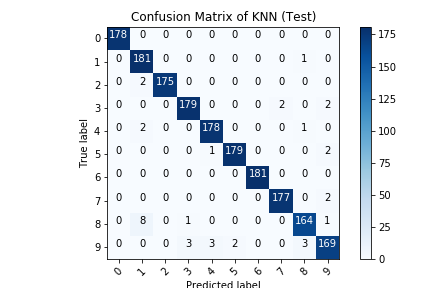
\includegraphics[width=3in]{knntest.png}
		\caption{Confusion Matrix of Test set (knn).}
		\label{fig:knntest}
	\end{center}
\end{figure} 
\newpage
\textbf{Decision tree hyper-parameters tuning:} We selected the maximum depth of decision tree based on validation accuracy, and corresponding metric will be printed on terminal (lines 159-187).\\*

\textbf{Training with best max\_depth on the whole training set:} We train on whole data and report confusion matrix of train set (lines 190-201). It is shown in Figure \ref{fig:dtreetrain}. This part of source code will output train time and confusion matrix on terminal.
\begin{figure}[h] 
	\begin{center}
		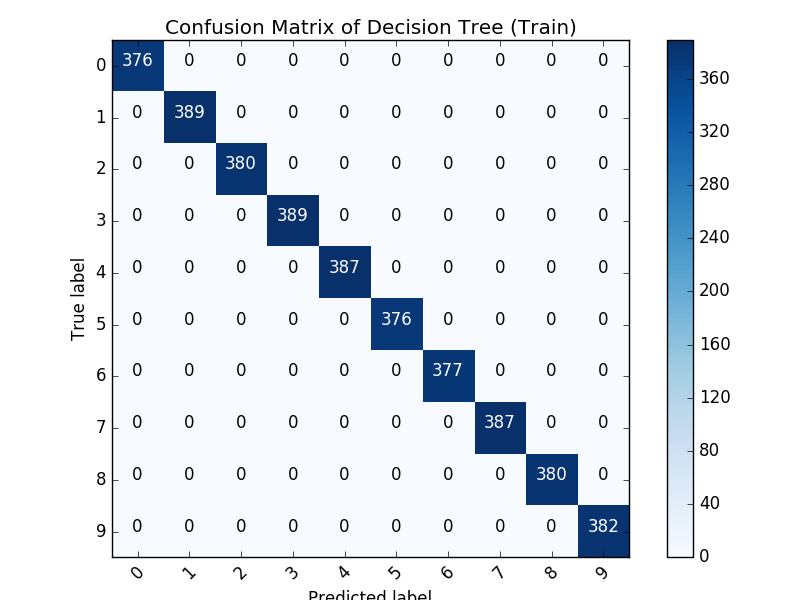
\includegraphics[width=3in]{dtreetrain.png}
		\caption{Confusion Matrix of Train set (Decision tree).}
		\label{fig:dtreetrain}
	\end{center}
\end{figure} 

\textbf{Evaluating decision tree model on test set:} In lines 204-213, we predict test labels and report the metrics. Test set confusion matrix is shown in Figure \ref{fig:dtreetest}.
\begin{figure}[h] 
	\begin{center}
		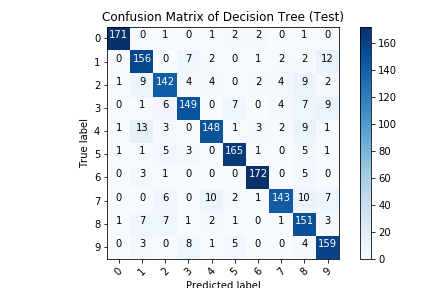
\includegraphics[width=3in]{dtreetest.png}
		\caption{Confusion Matrix of Test set (Decision tree).}
		\label{fig:dtreetest}
	\end{center}
\end{figure} 
\newpage
\textbf{Linear discrimination hyper-parameters tuning:} We selected the regularization strength of linear classifier based on validation accuracy, and corresponding metric will be printed on terminal (lines 224-252).\\*

\textbf{Training with best alpha on the whole training set:} We train on whole data and report confusion matrix of train set (lines 255-265). It is shown in Figure \ref{fig:sgdtrain}. This part of source code will output train time and confusion matrix on terminal.\\*
\begin{figure}[ht] 
	\begin{center}
		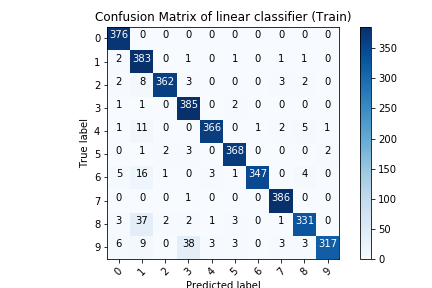
\includegraphics[width=3in]{sgdtrain.png}
		\caption{Confusion Matrix of Train set (linear classifier).}
		\label{fig:sgdtrain}
	\end{center}
\end{figure} 
\textbf{Evaluating linear discrimination model on test set:} In lines 268-277, we predict test labels and report the metrics. Test set confusion matrix is shown in Figure \ref{fig:sgdtest}.
\begin{figure}[ht] 
	\begin{center}
		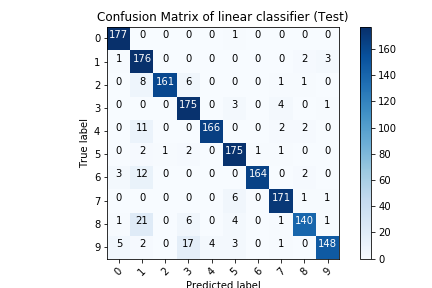
\includegraphics[width=3in]{sgdtest.png}
		\caption{Confusion Matrix of Test set (linear classifier).}
		\label{fig:sgdtest}
	\end{center}
\end{figure} 
\newpage
\textbf{MLP hyper-parameters tuning:} We selected the best parameters of neural network classifier (number of hidden layers, layer sizes, and regularization strength) based on validation accuracy, and corresponding metrics will be printed on terminal (lines 290-320).\\*

\textbf{Training with best parameters on the whole training set:} We train on whole data and report confusion matrix of train set (lines 323-335). It is shown in Figure \ref{fig:mlptrain}. This part of source code will output train time and confusion matrix on terminal.\\*
\begin{figure}[h] 
	\begin{center}
		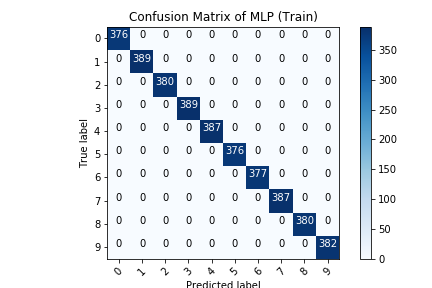
\includegraphics[width=3in]{mlptrain.png}
		\caption{Confusion Matrix of Train set (MLP).}
		\label{fig:mlptrain}
	\end{center}
\end{figure} 
\textbf{Evaluating neural network model on test set:} In lines 338-349, we predict test labels and report the metrics. Test set confusion matrix is shown in Figure \ref{fig:mlptest}.
\begin{figure}[ht] 
	\begin{center}
		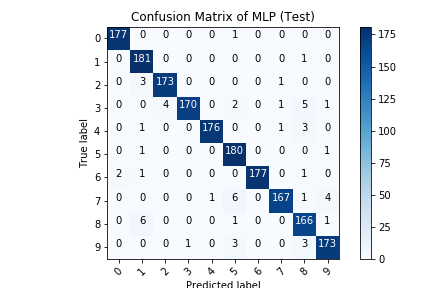
\includegraphics[width=3in]{mlptest.png}
		\caption{Confusion Matrix of Test set (MLP).}
		\label{fig:mlptest}
	\end{center}
\end{figure} 

\newpage
\textbf{Q2)} In all models except linear discrimination, accuracy per class on train set are 100\%. For knn the best k is equal 1, so its accuracy on train set must be 100\%, regarding decision tree there might be over-fitting as the validation and train accuracy differ by 8\%. Thus, as a result test accuracy is even worse, 85.5\%. we could reduce the effect of over-fitting by cross validation. Furthermore, when we look at MLP accuracies, 100\%, 99.4\%, 96.8\%, train, validation, and test respectively, we can conclude that there is not over-fitting. In addition, linear discrimination accuracies shows that it is not capable of achieving state-of-the-art results. Looking at all confusion matrix, we observed that class 8 is miss-classified as class 1 the most.\\*
In terms of training time, the fastest classifier is knn, because it does not have any operation in training time and simply store the data, and the slowest model is neural network, because it has many matrix multiplication during forward pass and back-propagation. In test time, decision tree is the fastest model, and slowest model is knn because it compare each test set with all instances in training set.\\\\

\textbf{Q3)} Source code (382-409) identifies misclassified instances for each model and prints the results on Terminal. We are supposed to eliminate 10\% of training instances, however the percentage of noisy data is less than 10\% (we didn't shuffle the data), thus we remove all of those data from training set that are mislabeled (about 5\%). Finally, we randomly split new reduced training data into 90\% train, and 10\% validation and repeat all the process which are asked in \textbf{Q1}. We reference the related lines in source code and provide confusion matrix figures in the rest of this report.

\textbf{knn hyper-parameters tuning with train data after removal:} Best k is selected based on validation accuracy, and corresponding metric will be printed on terminal (lines 424-452).\\*

\textbf{Training with best k on the whole training set after removal:} We train on whole data and report confusion matrix of train set (lines 456-465). It is shown in Figure \ref{fig:reknntrain}. This part of source code will output train time and confusion matrix on terminal.
\begin{figure}[ht] 
	\begin{center}
		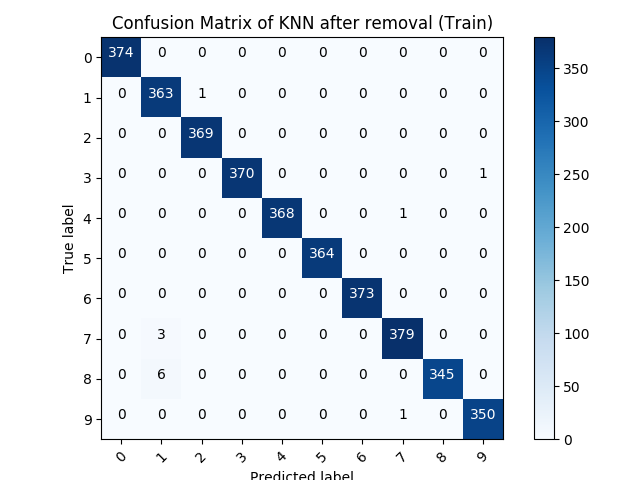
\includegraphics[width=3in]{reknntrain.png}
		\caption{Confusion Matrix of Train set after removal (knn).}
		\label{fig:reknntrain}
	\end{center}
\end{figure} 

\textbf{Evaluating knn model on test set:} In lines 469-478, we predict test labels and report the metrics. Test set confusion matrix is shown in Figure \ref{fig:reknntest}.
\begin{figure}[ht] 
	\begin{center}
		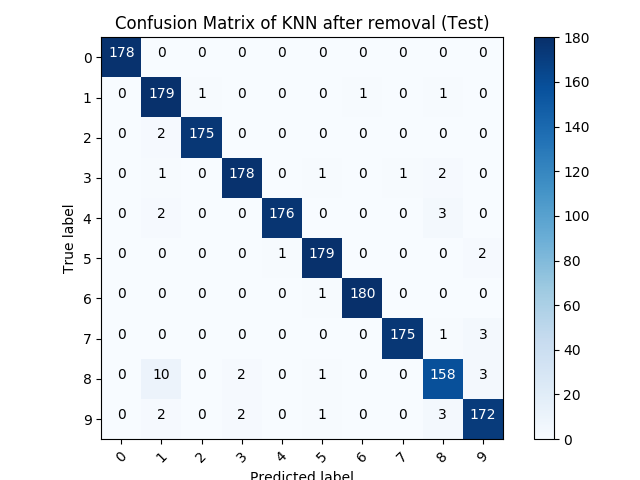
\includegraphics[width=3in]{reknntest.png}
		\caption{Confusion Matrix of Test set after removal(knn).}
		\label{fig:reknntest}
	\end{center}
\end{figure} 
\newpage
\textbf{Decision tree hyper-parameters tuning after removal:} We selected the maximum depth of decision tree based on validation accuracy, and corresponding metric will be printed on terminal (lines 491-520).\\*

\textbf{Training with best max\_depth on the whole training set after removal:} We train on whole data and report confusion matrix of train set (lines 523-534). It is shown in Figure \ref{fig:redtreetrain}. This part of source code will output train time and confusion matrix on terminal.
\begin{figure}[ht] 
	\begin{center}
		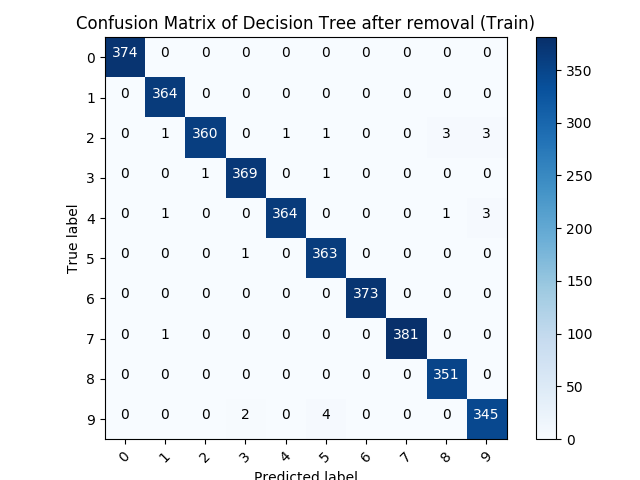
\includegraphics[width=3in]{redtreetrain.png}
		\caption{Confusion Matrix of Train set after removal (Decision tree).}
		\label{fig:redtreetrain}
	\end{center}
\end{figure} 

\textbf{Evaluating decision tree model on test set after removal:} In lines 537-546, we predict test labels and report the metrics. Test set confusion matrix is shown in Figure \ref{fig:redtreetest}.
\begin{figure}[ht] 
	\begin{center}
		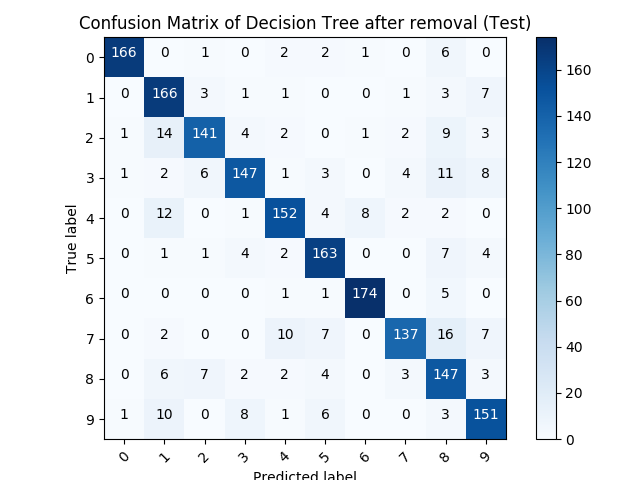
\includegraphics[width=3in]{redtreetest.png}
		\caption{Confusion Matrix of Test set after removal (Decision tree).}
		\label{fig:redtreetest}
	\end{center}
\end{figure} 
\newpage
\textbf{Linear discrimination hyper-parameters tuning after removal:} We selected the regularization strength of linear classifier based on validation accuracy, and corresponding metric will be printed on terminal (lines 558-586).\\*

\textbf{Training with best alpha on the whole training set after removal:} We train on whole data and report confusion matrix of train set (lines 589-599). It is shown in Figure \ref{fig:resgdtrain}. This part of source code will output train time and confusion matrix on terminal.\\*
\begin{figure}[ht] 
	\begin{center}
		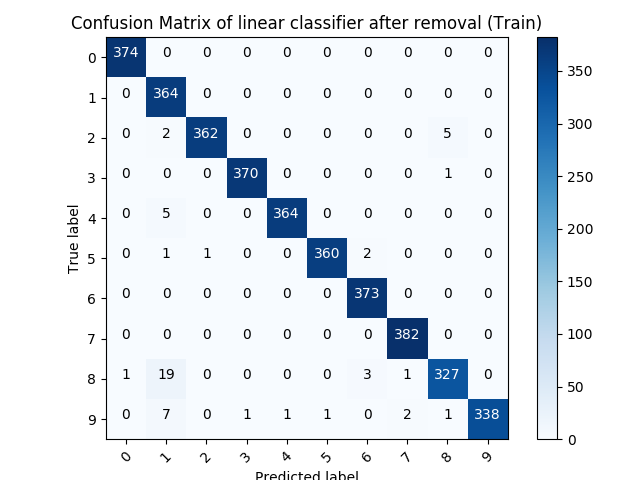
\includegraphics[width=3in]{resgdtrain.png}
		\caption{Confusion Matrix of Train set after removal (linear classifier).}
		\label{fig:resgdtrain}
	\end{center}
\end{figure} 
\textbf{Evaluating linear discrimination model on test set after removal:} In lines 602-611, we predict test labels and report the metrics. Test set confusion matrix is shown in Figure \ref{fig:resgdtest}.
\begin{figure}[ht] 
	\begin{center}
		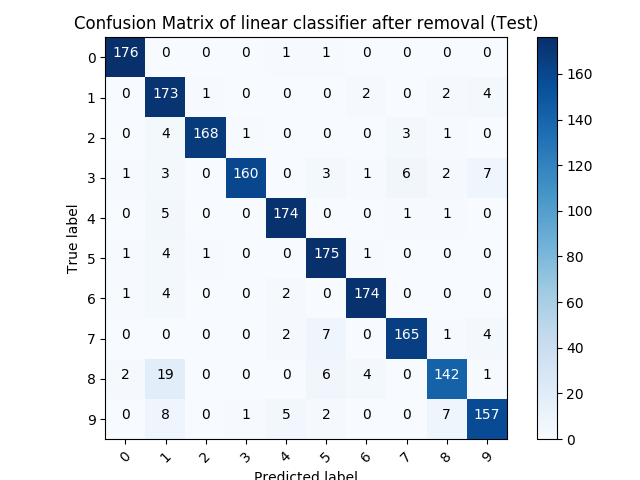
\includegraphics[width=3in]{resgdtest.png}
		\caption{Confusion Matrix of Test set after removal (linear classifier).}
		\label{fig:resgdtest}
	\end{center}
\end{figure} 
\newpage
\textbf{MLP hyper-parameters tuning after removal:} We selected the best parameters of neural network classifier (number of hidden layers, layer sizes, and regularization strength) based on validation accuracy, and corresponding metrics will be printed on terminal (lines 624-654).\\*

\textbf{Training with best parameters on the whole training set after removal:} We train on whole data and report confusion matrix of train set (lines 657-69). It is shown in Figure \ref{fig:remlptrain}. This part of source code will output train time and confusion matrix on terminal.\\
\begin{figure}[h] 
	\begin{center}
		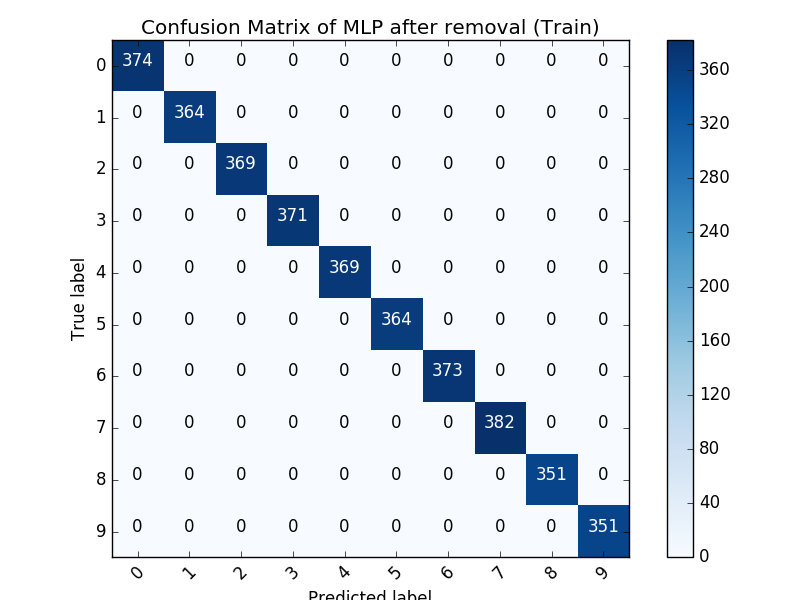
\includegraphics[width=3in]{remlptrain.png}
		\caption{Confusion Matrix of Train set after removal (MLP).}
		\label{fig:remlptrain}
	\end{center}
\end{figure} 
\textbf{Evaluating neural network model on test set after removal:} In lines 672-683, we predict test labels and report the metrics. Test set confusion matrix is shown in Figure \ref{fig:remlptest}.\\
\begin{figure}[ht] 
	\begin{center}
		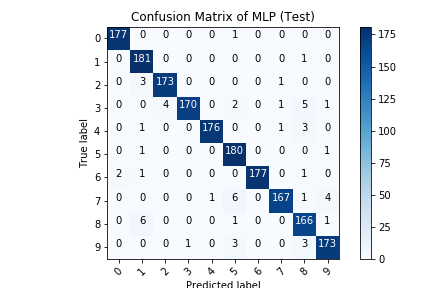
\includegraphics[width=3in]{mlptest.png}
		\caption{Confusion Matrix of Test set after removal (MLP).}
		\label{fig:remlptest}
	\end{center}
\end{figure}
\newpage 
Finally we compare the accuracy per classes of test data before and after removal for all models (lines 692-711). As it is shown in Figure \ref{fig:acc}, in our experiments, some classes accuracies get better and some get worse. Considering overall accuracy of models, decision tree model get better, and others decreased. However, performance of classifiers on test data set only changed less than 1\%. 

\begin{figure}[ht] 
	\begin{center}
		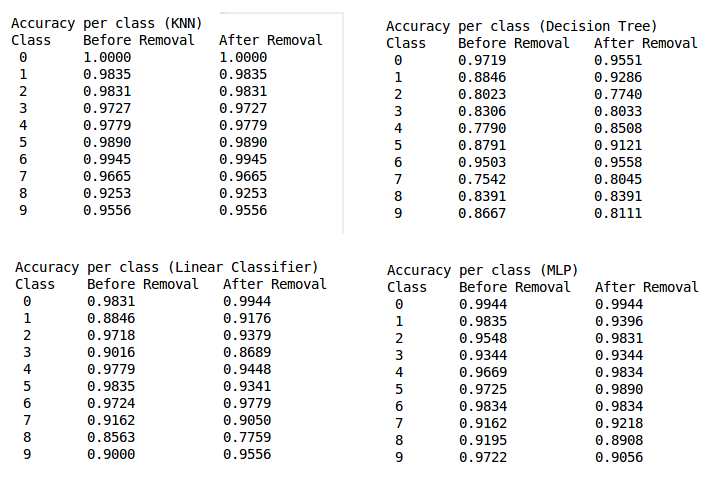
\includegraphics[width=6in]{acc.png}
		\caption{Test accuracy of models per class, before and after removal.}
		\label{fig:acc}
	\end{center}
\end{figure} 

\end{document}